Das Protokoll wird grundlegend mit zwei verschiedenen
Compilereinstellungen getestet. Dies sind die Geschwindigkeits- (\glqq O$2$
\grqq) und die Quellcodegrößenoptimierung (\glqq Os \grqq). 
\newline
% Hypothese 1
Dabei ist die Laufzeit bei O$2$ stets kleiner als bei Os. Weiterhin sollte der
Zeitbedarf bei größerwerdenden Datenpekten kontinuierlich ansteigen.
\newline
% Methodik 1
Dabei wurde untersucht, wie lange das Protokoll für die Verarbeitung von Texten
verschiedener Größe benötigt, die keine relevanten Bereiche besitzen. Dafür
wurden Dateien mit verschiedenen Größen von $2$ Bytes bis $10$ Millionen Byte 
angelegt, durch das Programm eingelesen und der Schnittstelle des Protokolls
übergeben. Vor der Übergabe der Daten wurde das Modul gelöscht und neu erstellt.
Dadurch ist ein Messen der reinen Verarbeitungsdauer gewährleistet. Für einen
aussagekräftigeren Wert und um potentielle Messungenauigkeiten zu kompensieren,
werden die Messungen für jede Einstellung $10$ Mal wiederholt und der Mittelwert
gebildet.
% Auswertung 1
\newline
Die Abbildung \ref{fig:diagrammInitial_worp} zeigt grafisch die Ergebnisse der
Messreihen für den initialen Durchlauf ohne relevante Bereiche. Dabei ist die
Laufzeit in $\mu s$ über die Textgröße in Byte logarithmisch aufgetragen. Für
relativ kleine Textgrößen hat die Geschwindigkeitsoptimierung noch keinen großen
Einfluss. Erst bei einer Größe von $5.000.000$ ($99\ \mu s$) oder
$10.000.000$ ($122\ \mu s$) Byte ist der erwartete Geschwindigkeitsprofit zu
verzeichnen.

\begin{figure}[H]
	\centering
	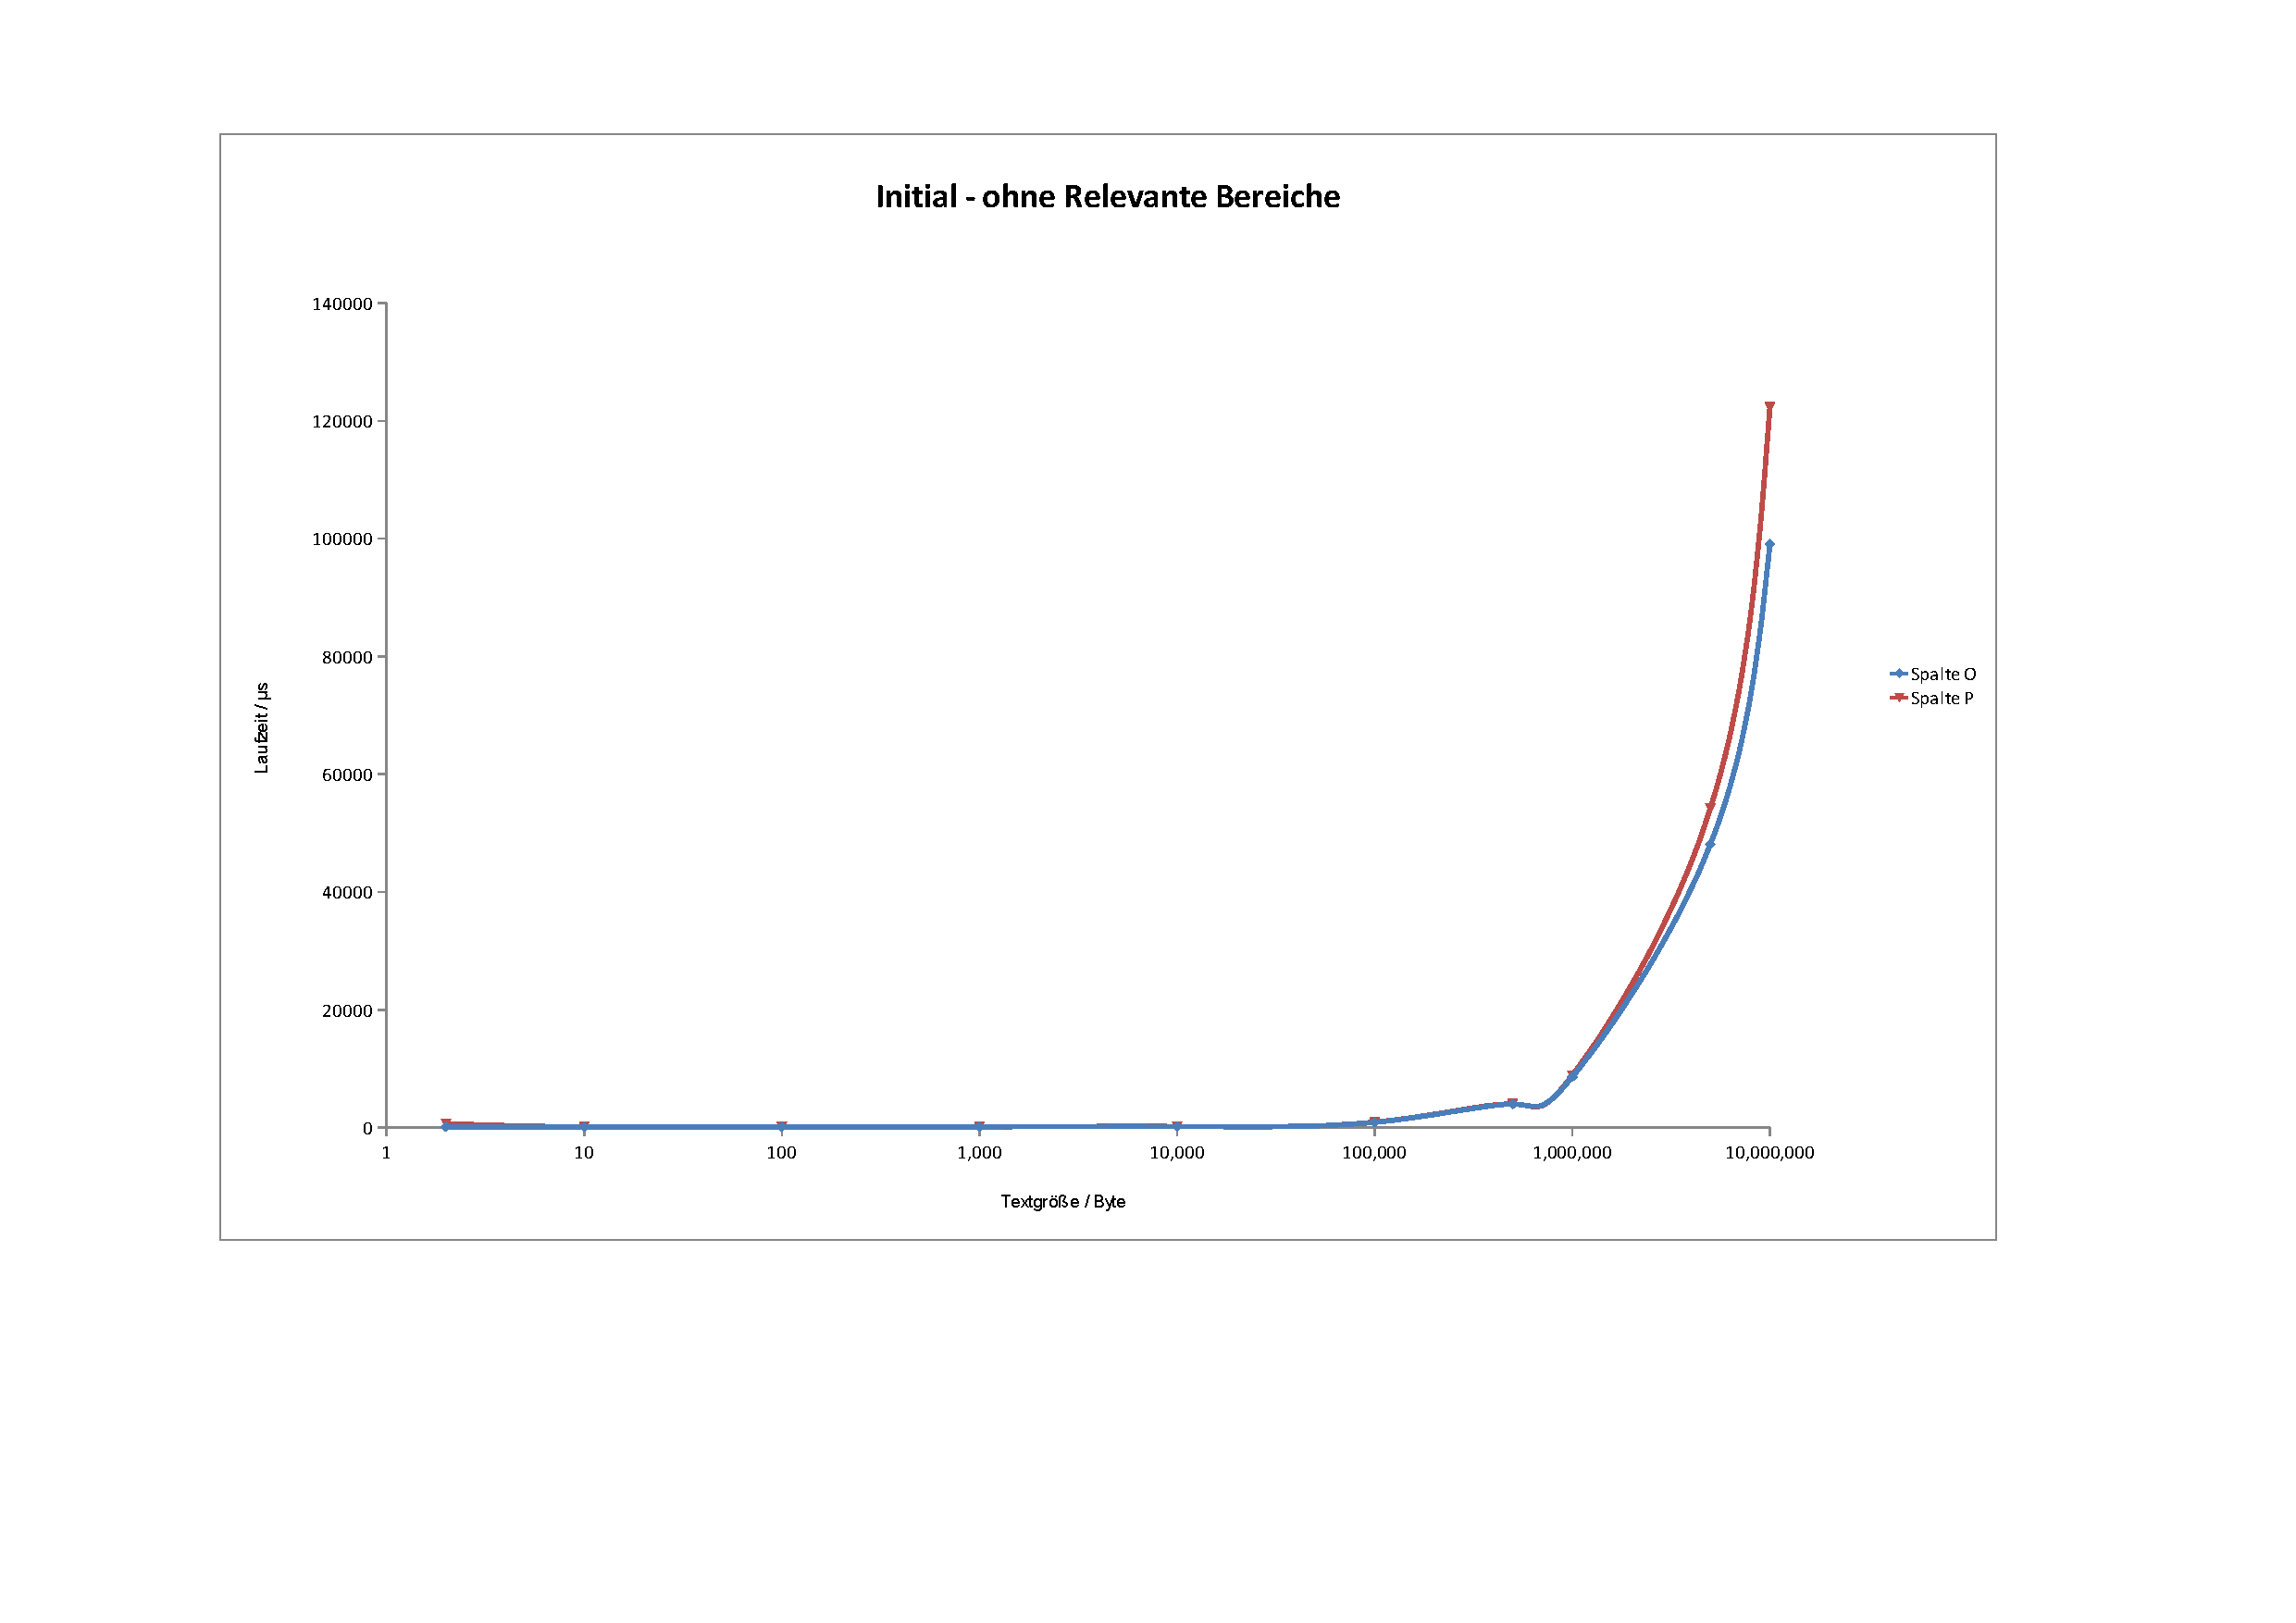
\includegraphics[scale=.45]{DiagrammInitial_worp.pdf}
	\label{fig:diagrammInitial_worp}
	\caption{Messung-Initial ohne relevante Bereiche}
\end{figure}

Der Nachteil gegenüber der Quellcodegrößenoptimierung liegt darin, dass
mehr Speicherplatz in Anspruch genommen wird, wodurch der
Geschwindigkeitsvorteil erreicht werden kann.
Die Wahl der jeweiligen Optimierungsmöglichkeit ist situationsabhängig. Auf dem
Mars stehen weniger Speicherressourcen zur Verfügung, wodurch eine
Geschwindigkeitsoptimierung weniger sinnvoll erscheint. Die gleichen
Betrachtungen ergeben sich für alle anderen Messreihen (Abbildung im Anhang
\ref{sec:Diagramme}). 

%Hypothese 2
Unter der Betrücksichtigung relevanter Bereiche ist eine Änderung der Laufzeit
anzunehmen. Diese sollte mit wachsender Anzahl an relevanten Bereichen steigen,
da zusätzlichen Berechnungen, die zum Zerteilen des Textes notwendig sind,
anfallen.
% Methodik 2
\newline
Zum Testen wird hier ein Text mit konstanter Größe von $5.000.000$ Byte
herangezogen. Dieser beinhaltet je nach Messreihe unterschiedlich viele
relevante Bereiche, von $1$ bis $1.000$. Auch hier wurde das Modul vor jeder
Messung zurückgesetzt.
% Auswertung 2
\newline
In Abbildung \ref{fig:diagrammInitial_wrp} ist die Laufzeit bezüglich
verschiedener Anzahlen relevanter Bereiche dargestellt. Die Textgröße bleibt
dabei stetig bei $5.000.000$ Byte. Damit ist ein Vergleich der Werte mit den
durchschnittlichen Werten der gleichen Textgröße aus Abbildung
\ref{fig:diagrammInitial_worp} möglich. Für nur wenige relevante Bereiche
unterscheiden sich die Werte marginal. Steigt die Anzahl, nimmt die Laufzeit
jedoch exponentiell zu (siehe Abbildung \ref{fig:diagrammInitial}) und bewegt
sich dann im Millisekunden-Bereich. Dies bedeutet, dass die Implementierung noch
nicht für die Verwendung von einer sehr großen Anzahl an relevanten Bereichen
optimiert wurde. Im Kapitel \ref{sec:Anwendungsszenarien} wurden bereits
mögliche Anwendungsszenarien betrachtet, welche ebenso mit wenigen relevanten
Bereichen auskommen. Dadurch ist eine Optimierung an dieser Stelle vorerst
nebensächlich.

\begin{figure}[H]
	\centering
	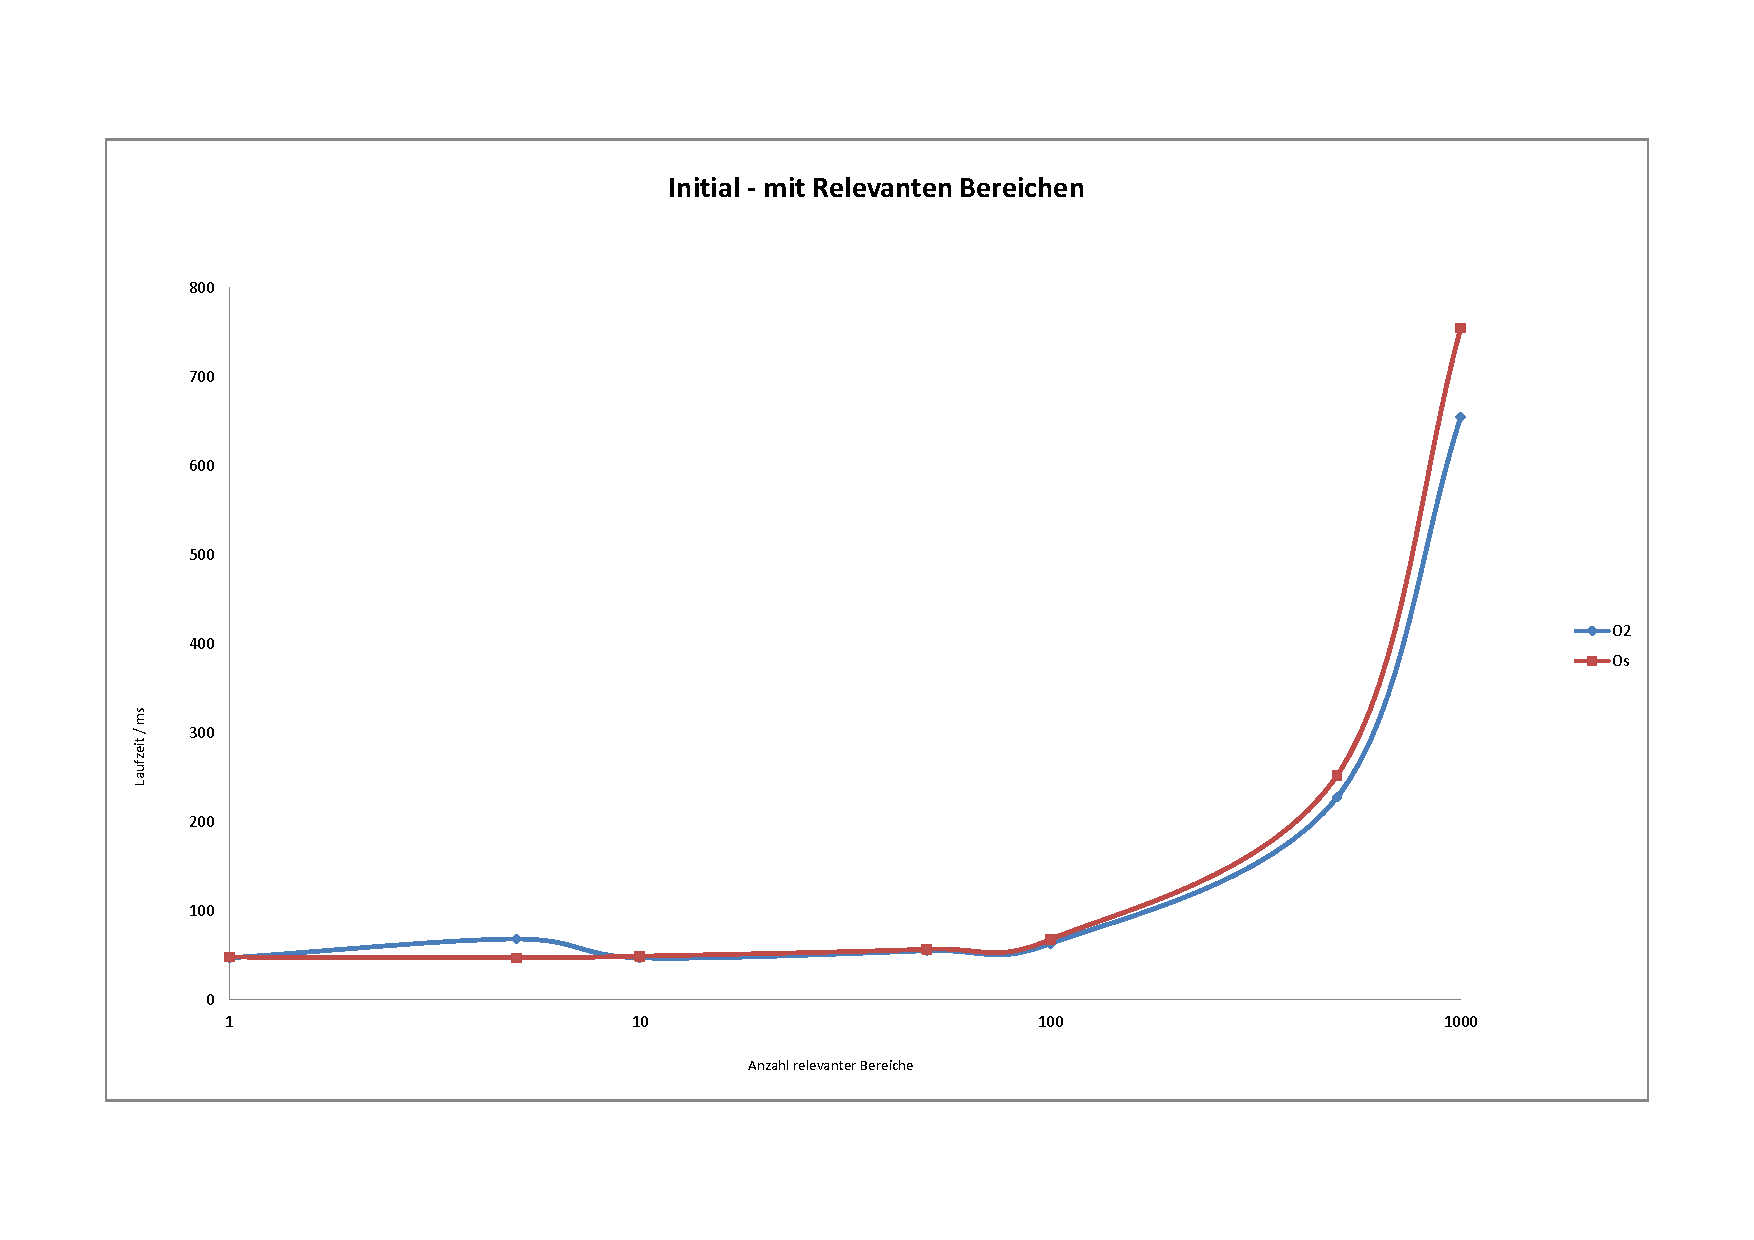
\includegraphics[width=\textwidth]{DiagrammInitial_wrp.pdf}
	\label{fig:diagrammInitial_wrp}
	\caption{Messung-Initial mit relevanten Bereichen}
\end{figure}

% Hypothese 3
Die bisherigen Untersuchungen wurden jedesmal auf Grundlage des Zurücksetzens
des Moduls betrachtet. Das Messen mit durchgängiglaufendem Modul ergibt Probleme
hinsichtlich des Speicherbedarfs. 
% Methodik 3
\newline
Die bisherigen Messungen werden nocheinmal ohne Zurücksetzen wiederholt. Dabei
werden relevante und nicht relevante Bereiche jeweils $10$ Mal vom Modul
verarbeitet (Verweis auf Anhang \ref{sec:messtabellen}), um eine möglichst größe
Datenmenge verarbeiten zu können WATN SCEIß AUSDRUCK!!!
% Auswertung 3
\newline
Hierbei ist zu
erkennen, dass die Verarbeitungsdauer ansteigt, je mehr Daten schon bearbeitet
wurden. Eine genauere Analyse zeigt, dass das Einsortieren in die priorisierende
\gls{FIFO} der Grund für die Laufzeitverlängerung ist. Bei diesem Testdurchlauf
wurden insgesamt $41.400$ Datenblöcke aus $548$ MB verarbeitet.
Dabei lagen alle Datenblöcke gleichzeitig in der \gls{FIFO}, wodurch das
Einsortieren neuer Blöcke sehr viel Rechenleistung in Anspruch nimmt.
Gleichzeitig werden diese Daten im Arbeitsspeicher und auf der Festplatte
gespeichert. Hierbei gilt zu untersuchen, ob diese Form der Datensicherung bei
einem Rover auf dem Mars praktikabel ist, da dieser über sehr begrenzte
Speicherressourcen verfügt. Alternativ müssen neue Methoden gefunden werden, den
Speicherverbrauch einzuschränken. So besteht die Möglichkeit, die Daten nur auf
der Festplatte zu speichern und in der \gls{FIFO} die Indizes zu diesen zu
hinterlegen, wodurch der Speicherverbrauch im Arbeitsspeicher stark reduziert
werden kann. Allerdings ist diese Methode bei sehr vielen Daten nicht optimal,
welche sich bei sehr langen Zeiträumen, in denen nicht gesendet werden kann,
ansammeln. Eine bessere Möglichkeit wäre, anhand einer \gls{TTL} (siehe Kapitel
\ref{sec:Vorueberlegung}) unrelevante Daten nur sehr kurzfristig vorzuhalten,
damit mehr Raum für Daten von hoher Relevanz ist.


% Die eben vorgestellten Messungen wurden auf zwei verschiedenen Wegen
% aufgenommen. Diese unterscheiden sich dahingehend, dass das Modul vor dem Erhalt
% neuer Daten gelöscht und anschließend neu erstellt wurde. Somit sind alle
% Datenstrukturen bei jedem Messdurchgang leer, wodurch vor allem die Komplexität
% der Einsortierung in die priorisierende \gls{FIFO} verringert wurde. Für den
% zweiten Fall wurden die Daten alle nacheinander verschickt, um ein realistischeres
% Szenario darstellen zu können.

% Die Messreihen sind der besseren Übersicht halber
% nocheinmal im Anhang dargestellt (\ref{sec:messtabellen}).
 


